\subsection{\secState{R}Architecture}\label{sec:utmArchitecture}
\paragraph{UTM concept} is based on \emph{asynchronous event-based control} \cite{zimmer2011rule}. \emph{Event} in \emph{controlled airspace} is handled in form of \emph{cases} \cite{prevot2016uas}. There are following \emph{event sources}:

\begin{enumerate}
    \item \emph{Weather Information Service} (from \cite{zimmer2014selective}) - used to create \emph{weather case} (tab. \ref{tab:weatherConstraint}).
    
    \item \emph{Position Notification from UAS systems} (tab. \ref{tab:positionNotification}) - used to create \emph{collision cases} (new functionality) (tab. \ref{tab:collisionCase}).
\end{enumerate}


\paragraph{Decision frame} (eq. \ref{eq:decisionFrameDefinition}). The \emph{UTM} is operating in discrete decision frames which are starting on current \emph{decision time} and ending at  next \emph{decision  time}:

\begin{equation}\label{eq:decisionFrameDefinition}
    decision Frame_i = [decision Time_i, decision Time_{i+1}[,\quad i \in {1,\dots,k}, k \in \N^+
\end{equation}

\paragraph{Event based airspace control} is collecting  events in  previous $decisionFrame_{i-1}$ and issuing commands in current $decisionFrame_i$.There are following phases during the \emph{UTM frame} cycle:
\begin{enumerate}
    \item \emph{Planning} - the detection phase, when the hazardous situations are assessed.
    
    \item \emph{Fulfillment} - the monitoring phase, when the state of affairs for directives and mandates is full filled by controlled UAS systems. 
    
    \item \emph{Acknowledgement} - the closing phase, when UTM assess and acknowledges the performance of controlled UAS systems.
\end{enumerate}


\begin{figure}[H]
    \centering
    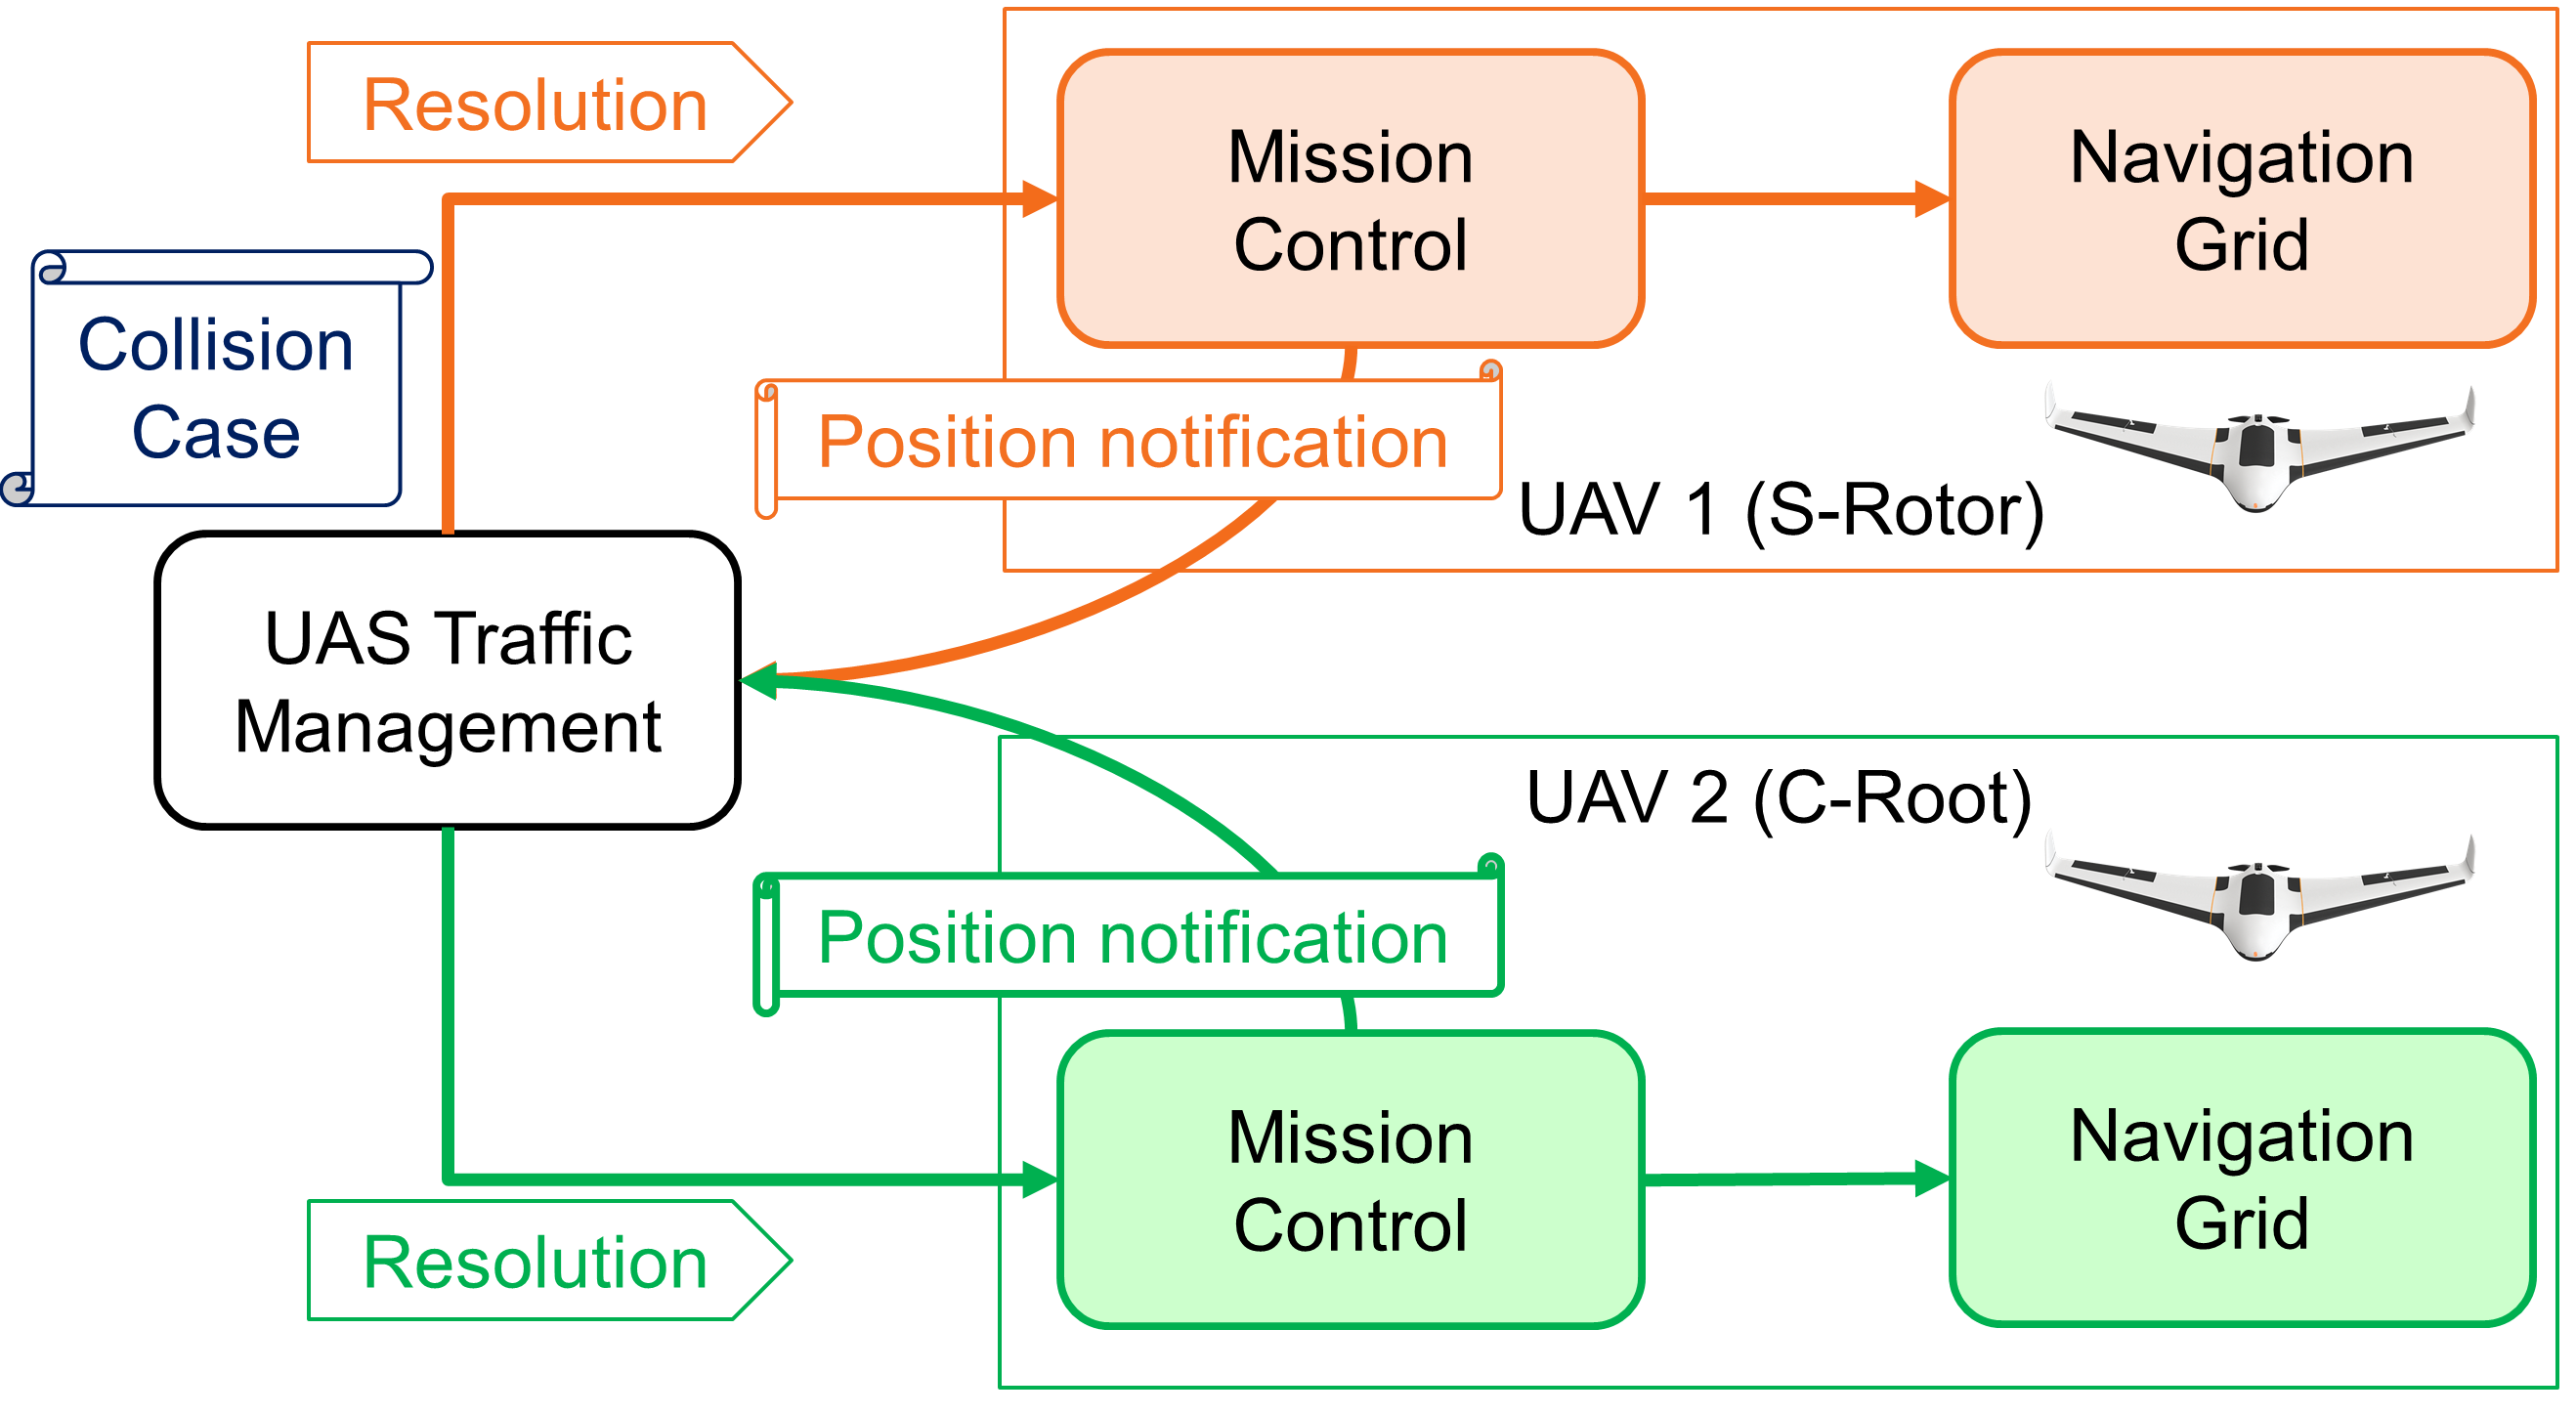
\includegraphics[width=0.7\linewidth]{\FIGDIR/RE002UTMCommunicationDiagram} 
    \caption{UAS Traffic Management (UTM) architecture overview.}
    \label{fig:UTMArchitectureOverview}
\end{figure}

\paragraph{Architecture:} (fig. \ref{fig:UTMArchitectureOverview}).  There are multiple UAS systems equipped with standard \emph{Mission Control} and \emph{Navigation} procedures. 

Depending on the \emph{airspace cluster} decision time frame they are sending \emph{periodical position notifications} (tab. \ref{tab:positionNotification}).

The \emph{UAS Traffic Management} (UTM) collects the event data from \emph{Weather Information Service} and \emph{Position Notifications} calculating respective \emph{cases}. 

If there is an \emph{active collision/weather case} the \emph{UTM} will send \emph{resolutions} to respective airspace attendants. 